\chapter{Architektura odbiornika}

\section{Wstęp}
Wszechstronność systemu była jednym z wymogów projektowych architektury odbiornika. 
Dostosowanie do różnych rodzajów modulacji, pasm częstotliwości i mocy odbieranego sygnału nie powinno powodować zmian w konfiguracji sprzętowej.
Jednostką zarządzającą działaniem odbiornika będzie komputer PC.
Również na nim miejsce będzie miała eliminacja zakłóceń, zatem moduł radiowy powinien posiadać interfejs o wysokiej przepustowości.

\section{Radio definiowane programowo}
Odpowiedzią na stawiane wymagania jest Radio Definiowane Programowo, w skrócie SDR od ang. \textit{Software Defined Radio}.
Dzięki zastosowaniu cyfrowych mieszaczy i filtrów urządzenie może zostać przeprogramowane do celów, których nikt nie przewidział na etapie projektowania systemu telekomunikacyjnego.
Stanowi pewne zabezpieczenie na wypadek zmiany koncepcji lub pojawienia się nowego standardu, ponieważ nie wymaga ingerencji w infastrukturę sprzętową, której modernizacja może przewyższać koszt SDR.
Radio programowalne pozwala na szybkie prototypowanie przy użyciu środowisk dostępnych na różnych systemach operacyjnych. 
Programy takie jak Matlab, Simulink, LabView lub wykorzystywany w tym projeckie GnuRadio, oferują łatwość użytkowania bez specjalistycznej wiedzy z zakresu archiektury procesorów sygnałowych. \cite{ImplementingSDR:92304} 

\section{USRP}
\subsection{Architektura}
Architektura SDR przedstawiona na Rysunku \ref{usrp_architecture} jest wspólna dla wszytkich produktów z rodziny USRP. Po przejściu przez wzmacniacz, sygnał analogowy trafia na demodulator kwadraturowy, który rozdziela jego składowe $I$ i $Q$. 
Widmo sygnałów w.cz. przeniesione zostaje do pasma podstawowego (BB) lub pośredniego (IF). 
Wtedy następuje konwersja analogowo- cyfrowa. 
USRP posiada po dwa przetworniki ADC na każdej lini TX/RX.
Układ FPGA realizuje funkcję konwertera DDC (ang. \textit{Digital Down Converter}), który ogranicza liczbę próbek wyprodukowanych przez ADC, zachowując informację niesioną przez sygnał.
Mniejsza przepływność bitowa pozwala na efektywne przesyłanie danych z USRP do komputera w celu dalszego przetwarzania. \cite{usrp_bw}

\begin{figure}
\centering
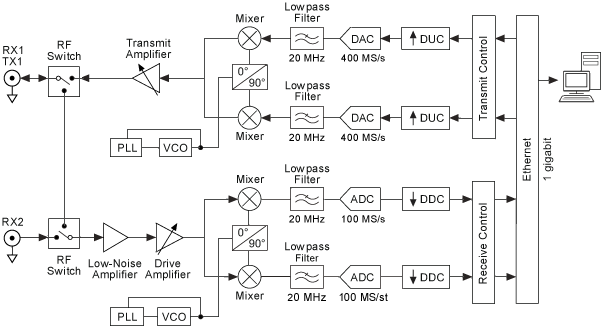
\includegraphics[scale=0.8]{ch4_usrp_architecture.png}
\caption{Architektura USRP}
\label{usrp_architecture}
\end{figure}

\subsection{Wybór właściwego USRP}
USRP występuje w wielu modelach, 

Pytania na które należało odpowiedzieć
\begin{enumerate}
\item Jaki jest wymagany zakres częstotliwości pracy odbiornika?
\item Jakiej szerokości pasmo odbiornik powinien odbierać?
\item Czy odbiornik będzie jednostką autonomiczną czy współpracującą z hostem (PC)?
\item Czy wymagana jest komunikacja dwukierunkowa (full duplex)?
\item Czy obsługiwany będzie tryb MIMO?
\end{enumerate}

\paragraph{Pasmo} 
\paragraph{Interfejs}



